% Generator: hand-authored TikZ schematic traced from the fixed source; triangle proportions are illustrative.
% Source ID: src-120ea104f8cb373f5731039fa9d36469df457869849f27420831962ef1ad2306
% PDF SHA-256: d0081500bd56d03199ddcf232fe8e870f2ecd7e9c41ba849417af9af79fbb702
% PDF page 2; printed page 125; question 19.
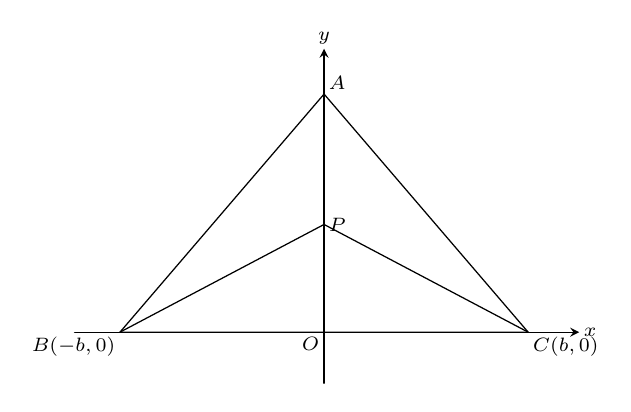
\begin{tikzpicture}[
  x=0.72cm,y=0.72cm,line width=0.45pt,line cap=round,>=stealth,
  every node/.style={font=\scriptsize,inner sep=1.5pt}
]
  \coordinate (O) at (0,0);
  \coordinate (A) at (0,4.2);
  \coordinate (P) at (0,1.9);
  \coordinate (B) at (-3.6,0);
  \coordinate (C) at (3.6,0);

  \draw[->] (-4.4,0)--(4.5,0) node[right] {$x$};
  \draw[->] (0,-0.9)--(0,5.0) node[above] {$y$};
  \draw (A)--(B)--(C)--cycle;
  \draw (P)--(B) (P)--(C);

  \node[above right] at (A) {$A$};
  \node[below left] at (B) {$B(-b,0)$};
  \node[below right] at (C) {$C(b,0)$};
  \node[below left] at (O) {$O$};
  \node[right] at (P) {$P$};
\end{tikzpicture}
